%% LyX 2.3.6.1 created this file.  For more info, see http://www.lyx.org/.
%% Do not edit unless you really know what you are doing.
\documentclass[twoside,english]{elsarticle}
\usepackage[T1]{fontenc}
\usepackage[latin9]{inputenc}
\pagestyle{headings}
\usepackage{url}
\usepackage{graphicx}
\usepackage{wasysym}

\makeatletter

%%%%%%%%%%%%%%%%%%%%%%%%%%%%%% LyX specific LaTeX commands.
%% Because html converters don't know tabularnewline
\providecommand{\tabularnewline}{\\}

%%%%%%%%%%%%%%%%%%%%%%%%%%%%%% User specified LaTeX commands.
% specify here the journal
\journal{MethodsX}

% use this if you need line numbers
%\usepackage{lineno}

\makeatother

\usepackage{babel}
\usepackage{listings}
\renewcommand{\lstlistingname}{Listing}

\begin{document}

\begin{frontmatter}{}

\title{OPTIMUS: a multidimensional global optimization package}

\author{Vasileios Charilogis}

\ead{v.charilog@uoi.gr}

\author{Ioannis G. Tsoulos\corref{cor1}}

\ead{itsoulos@uoi.gr}

\cortext[cor1]{Corresponding author}

\address{Department of Informatics and Telecommunications, University of Ioannina,
Greece}
\begin{abstract}
A variety of problems from many research areas can be modeled using
global optimization, such as problems in the area of image processing,
medical informatics, economic models, etc. This paper presents a programming
tool written in ANSI C++, which researchers can use to formulate the
problem to be solved and then make use of the local and global optimization
methods provided by this tool to efficiently solve such problems.
The main features of the proposed software are:\\
	\begin{enumerate}
		\item Ability to code the objective problem in a high level language such
as ANSI C++.

\item Incorporation of many global optimization techniques to solve the
objective problem.

\item Parameterization of global optimization methods using user-defined
parameters.
	\end{enumerate}
\end{abstract}
\begin{keyword}
Global optimization \sep Termination rules \sep Stochastic methods
\end{keyword}

\end{frontmatter}{}


\section*{Graphical abstract }

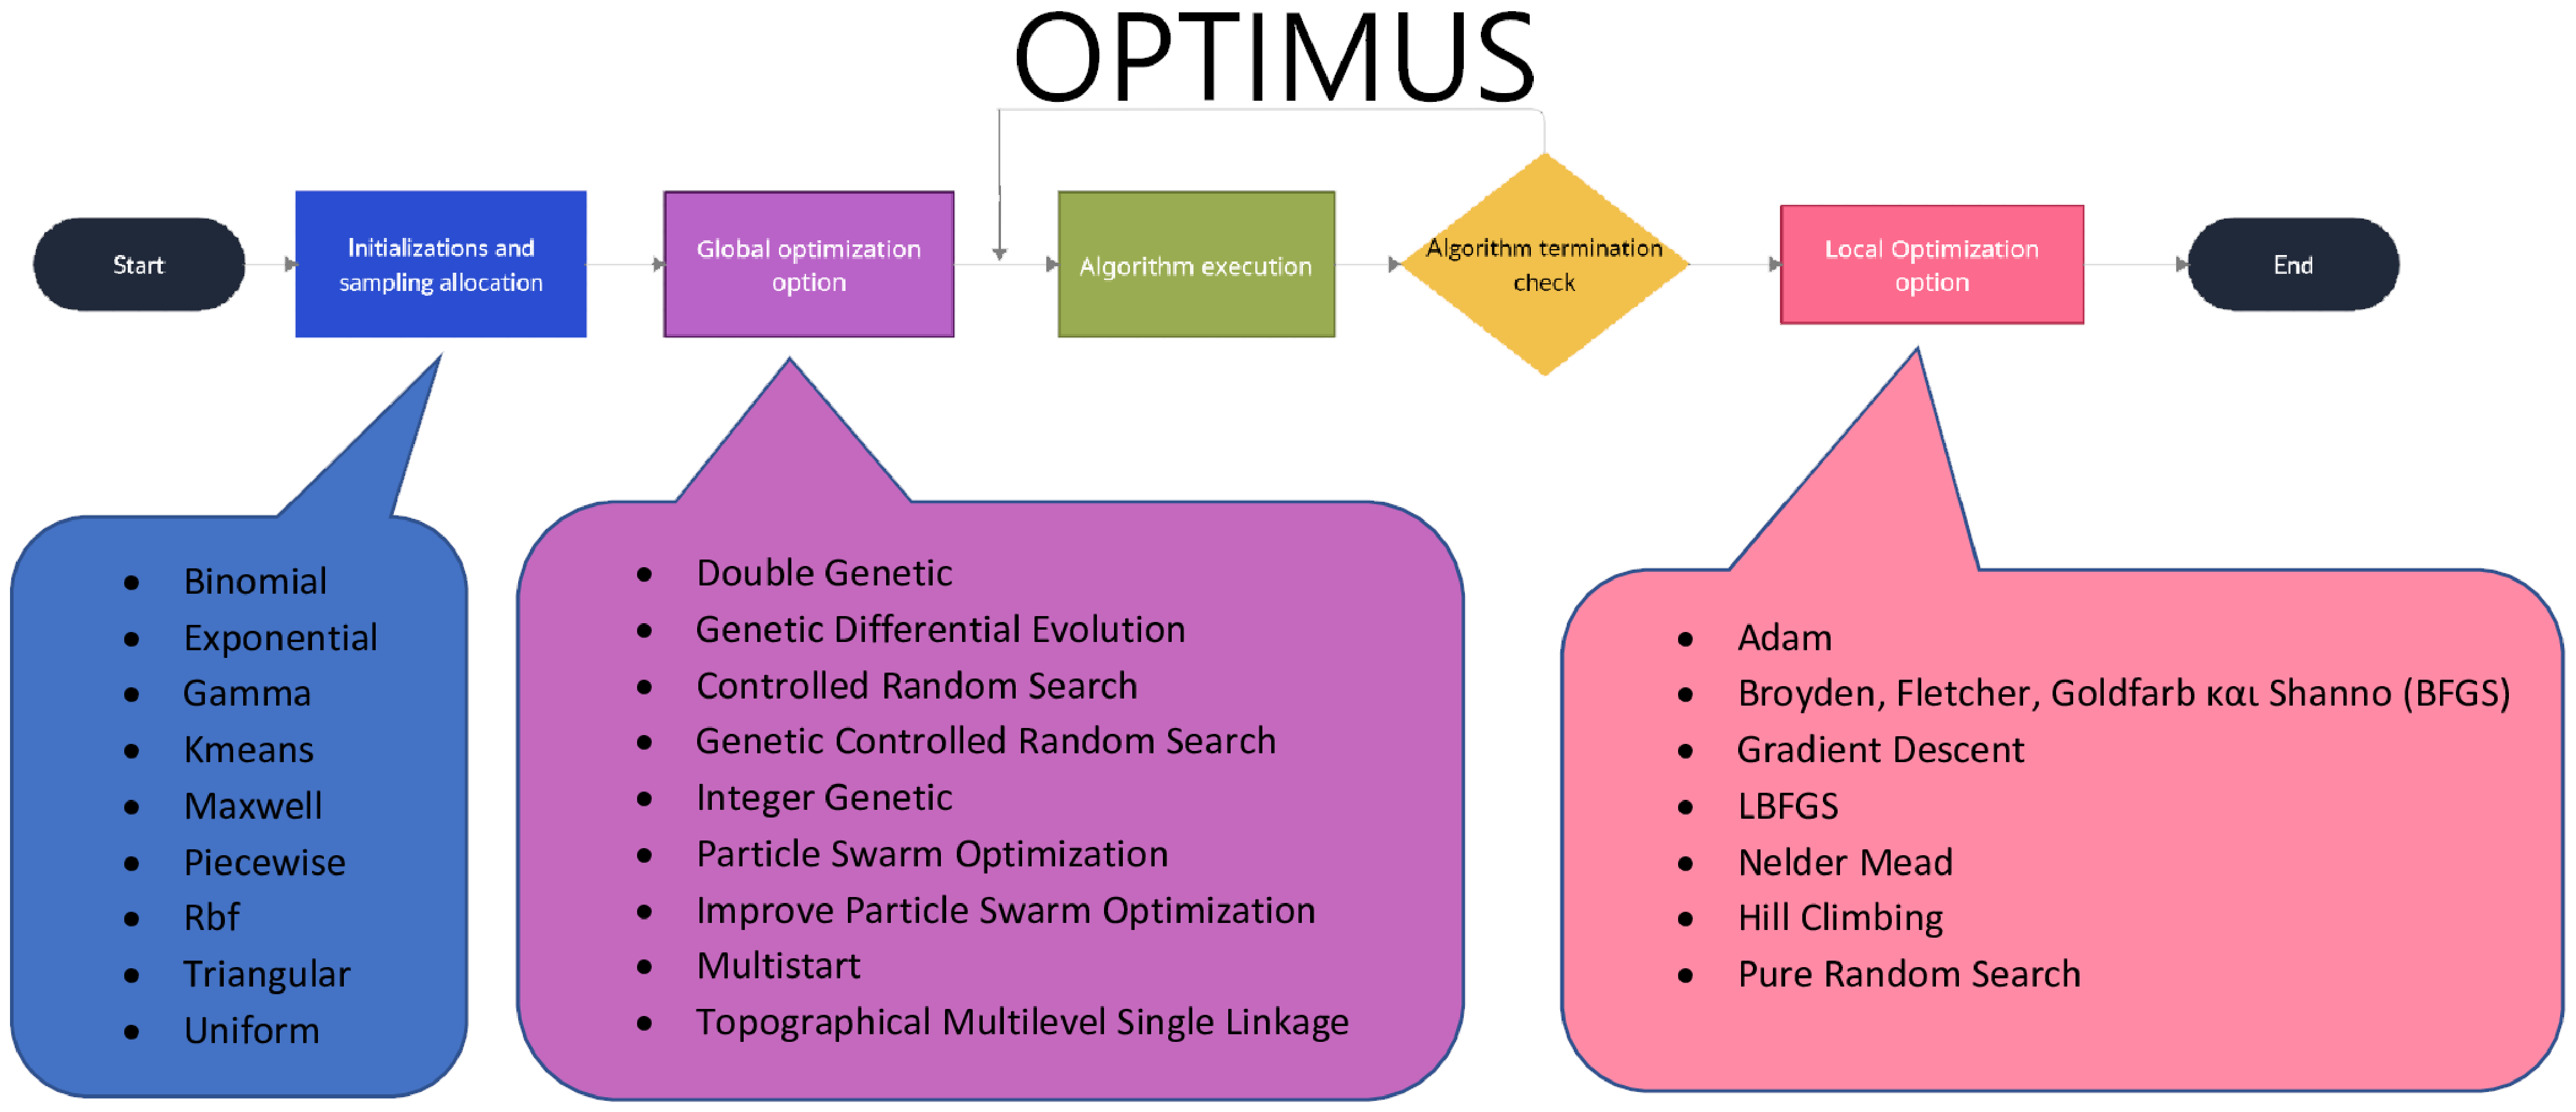
\includegraphics[scale=0.2]{optimus_abstract}

\section*{Specifications table}

\begin{tabular}{|c|c|}
\hline 
\textbf{Subject area} & Computer science\tabularnewline
\hline 
\textbf{More specific subject area} & Global Optimization\tabularnewline
\hline 
\textbf{Method name} & Optimus\tabularnewline
\hline 
\textbf{Name and reference of original method} & The software is proposed for first time.\tabularnewline
\hline 
\textbf{Resource availability} & \url{https://github.com/itsoulos/OPTIMUS/}\tabularnewline
\hline 
\end{tabular}

\section{Introduction}

The task of locating the global minimum of a continuous and differentiable
function $f:S\rightarrow R,S\subset R^{n}$ is defined as
\begin{equation}
x^{*}=\mbox{arg}\min_{x\in S}f(x)\label{eq:eq1}
\end{equation}
with $S$: 
\[
S=\left[a_{1},b_{1}\right]\otimes\left[a_{2},b_{2}\right]\otimes\ldots\left[a_{n},b_{n}\right]
\]
Methods that aim to locate the global minimum finds application in
economics \citep{globalecon1,globalecon2}, physics \citep{global_physics1,global_physics2},
chemistry \citep{global_chemistry1,global_chemistry2}, medicine \citep{global_med1,global_med2}
etc. Also, global optimization methods were used on some symmetry
problems \citep{go_symmetry0,go_symmetry1,go_symmetry2} as well as
on inverse problems \citep{global_nonlinear1,global_nonlinear2,global_nonlinear3}.
In the relevant literature there are a number of global optimization
techniques, such as Adaptive Random Search methods \citep{go_adaptive1,go_adaptive2},
Controlled Random Search methods \citep{go_crs1,go_crs2}, Simulated
Annealing \citep{go_sa1,go_sa2,go_sa3}, Genetic algorithms \citep{go_ga1,go_ga2},
Ant Colony Optimization \citep{go_ant1,go_ant2}, Particle Swarm Optimization
\citep{go_pso1,go_pso2} etc. Moreover, many hybrid techniques have
been proposed to tackle the global optimization problem, such as methods
that combine Particle Swarm Optimization and Genetic algorithms \citep{go_pso_genetic_hybrid1,go_pso_genetic_hybrid2},
methods that combine the Simplex method and Inductive search \citep{hybrid1}
etc. Because of the large demands that global optimization methods
have on computing power, several techniques have been proposed that
take advantage of modern parallel architectures \citep{gpu1,gpu2,gpu3}.

In this work, an integrated computing environment is proposed for
solving global optimization problems. In this the researcher can code
the objective function in the C++ programming language and then formulate
a strategy to solve the problem. In this strategy, the researcher
can choose from a series of sampling methods, choose a global minimization
method established in the relevant literature and possibly some local
minimization method to improve the produced result. Similar software
environments can be found, such as the BARON software package \citep{baron},
the MERLIN optimization software \citep{merlin}, the DEoptim software
\citep{deoptim} etc.

The rest of this article is organized as follows: in section \ref{sec:Software}
the software is described in detail, in section \ref{sec:Experiments}
some experiments are conducted to show the effectiveness of the proposed
software and finally in section \ref{sec:Conclusions} some conclusions
and guidelines for future work are presented.

\section{Software \label{sec:Software}}

The software is entirely written in ANSI C++ using the freely available
QT programming library, which can be downloaded from \url{https://qt.io}.
The user can code the objective problem in C++ by defining some critical
functions such as the dimension of the function or the objective function.
Subsequently, the user can select a global optimization method to
apply to the problem from a wide range of available methods. Also,
the user can extend the series of methods by adding some new method.\textbf{
}In the following subsections, the installation process of the proposed
software will be analyzed and a complete example of running an objective
problem will be given.

\subsection{Installation }

At the present time, the software package can only be installed on
computers with the Linux operating system, but in the future it will
be able to be installed on other systems as well. The instructions
to install the package on a computer are as follows:
\begin{enumerate}
\item Download and install the QT programming library from \url{https://qt.io }
\item Download the software from \url{https://github.com/itsoulos/OPTIMUS}
\item Set the \emph{OPTIMUSPATH} environment variable pointing at the installation
directory of OPTIMUS e.g. OPTIMUSPATH=/home/user/OPTIMUS/, where user
is the user name in the Linux operating system.
\item Set the \emph{LD\_LIBRAPY\_PATH} to include the OPTIMUS/lib subdirectory
e.g. LD\_LIBRAPY\_PATH=\$LD\_LIBRAPY\_PATH:\$OPTIMUSPATH/lib/:
\item Issue the command: cd \$OPTIMUSPATH 
\item Execute the compilation script:\emph{ ./compile.sh }
\end{enumerate}
After the compilation is complete, the \emph{lib} folder will contain
the supported global optimization methods in the form of shared libraries,
the \emph{PROBLEMS} folder will contain a number of example optimization
problems from the relevant literature, and the \emph{bin} folder will
contain the main executable of the software named \emph{OptimusApp}.
This executable can be used to apply global optimization techniques
to objective problems.

\subsection{Implemented global optimization methods }

In the following, the global optimization methods present in the proposed
software are presented. In most of them, a local optimization method
is applied after their end in order to find the global minimum with
greater reliability. In the proposed software, each implemented global
optimization method has a set of parameters that can determine the
global optimization path and the effectiveness of the method. For
example, the genetic algorithm contains parameters such as the number
of chromosomes or the maximum number of generations allowed. The implemented
global optimization methods are:
\begin{enumerate}
\item Differential Evolution. The differential evolution method is included
in the software as suggested by Storn\citep{de_main_paper} and denoted
as \textbf{de}. This global optimization technique has been widely
used in areas such as community detection \citep{de_symmetry1}, structure
prediction of materials \citep{de_symmetry3}, motor fault diagnosis
\citep{de_symmetry6}, automatic clustering techniques \citep{de_symmetry7}
etc.
\item Improved Differential Evolution. The modified Differential Evolution
method as suggested by Charilogis et al \citep{gende} is implemented
and denoted as \textbf{gende}.
\item Double precision genetic algorithm. A modified genetic algorithm \citep{doublepop_tsoulos}
is included in the software and it is denoted as \textbf{DoubleGenetic}.
Genetic algorithms are typical representatives of evolutionary techniques
with many applications such as scheduling problems \citep{genetic1},
the vehicle routing problem \citep{genetic2}, combinatorial optimization
\citep{genetic3}, architectural design etc \citep{genetic4}.
\item Integer precision genetic algorithm. The method denoted as \textbf{IntegerGenetic}
is a copy of the \textbf{DoubleGenetic} method, but with the usage
of integer values as chromosomes. This global optimization method
is ideal for problems such as the TSP problem \citep{tsp1,tsp2},
path planning \citep{pathPlanning}, Grammatical Evolution applications
\citep{ge} etc.
\item Improved Controlled Random Search. An improved version of Controlled
Random Search as suggested by Charilogis et al \citep{gcrs} is implemented
and it is denoted as \textbf{CCRS}.
\item Particle Swarm Optimization. A PSO variant denoted as \textbf{Pso}
is also included in the software. The particle swarm optimization
method was applied successfully in a vast number of problems such
as parameter extraction of solar cells \citep{psoApp1}, crystal structure
prediction \citep{psoApp2}, molecular simulations \citep{psoApp3}
etc.
\item Improved Particle Swarm Optimization. The improved Particle Swarm
method as suggested by Charilogis and Tsoulos \citep{ipso}. The implemented
method is denoted as \textbf{iPso}.
\item Multistart. A simple method that initiates local searches from different
initial points is also implemented in the software. Despite its simplicity,
the multistart method has been applied on many problems, such as the
TSP problem\textbf{ }\citep{multistart-tsp}, the vehicle routing
problem \citep{multistart-vehicle}, the facility location problem
\citep{multistart_fac}, the maximum clique problem \citep{multistart_clique},
the maximum fire risk insured capital problem \citep{multistart_fire},
aerodynamic shape problems \citep{multistart-aero} etc
\item Topographical Multi level single linkage. This method is proposed
by Ali et al \citep{tmlsl} and it is denoted as \textbf{Tmlsl} in
the implementation. 
\item The MinCenter method. In the software presented here, another multistart
method has been included, which forms, with the use of the K-Means
clustering algorithm, the regions of attraction for the local minima
of the objective problem. This method is denoted as \textbf{MinCenter}
and it was originally published by Charilogis and Tsoulos \citep{mincenter}.
\end{enumerate}

\subsection{Implemented local optimization methods}

The proposed software uses, in addition to global optimization methods
and local optimization methods, which can be used in most global minimization
techniques, with the $--$localsearch\_method parameter. The implemented
local optimization methods are the following:
\begin{enumerate}
\item The \textbf{bfgs} method. The Broyden\textendash Fletcher\textendash Goldfarb\textendash Shanno
(BFGS) algorithm was implemented using a variant of Powell \citep{powell}.
\item The \textbf{lbfgs} method. The limited memory BFGS method \citep{lbfgs}
is implemented as an approximation of the BFGS method using a limited
amount of computer memory. This local search procedure is ideal for
objective functions of higher dimensions.
\item The Gradient descent method. This method is denoted as \textbf{gradient}
in the software and implements the Gradient Descent local optimization
procedure. This local search procedure is used in various problems
such as neural network training \citep{gradient1}, image registration
\citep{gradient2} etc.
\item The \textbf{adam} method. The adam local optimizer \citep{Adam} is
implemented also.
\item The Nelder Mead method. The Nelder - Mead simplex procedure for local
optimization \citep{nelderMead} is also included in the software
and it is denoted as \textbf{nelderMead}.
\item Hill climbing. The hill climbing local search procedure denoted as
\textbf{hill} is also implemented. The method has been used in various
fields, such as design of photovoltaic power systems \citep{hill1},
load balancing in cloud computing \citep{hill2} etc. 
\end{enumerate}

\subsection{Objective problem deployment }

The objective problem must be coded in the C++ programming language.
The programmer must provide the software with a series of functions
that describe key components of the problem, such as the problem dimension,
the objective function, and the derivative.

\subsubsection{Objective function coding}

Figure \ref{fig:A-typical-representation} shows an objective function
written with the functions required by this software. This code is
used for the minimization of the Rastrigin function defined as:
\[
f(x)=x_{1}^{2}+x_{2}^{2}-\cos\left(18x_{1}\right)-\cos\left(18x_{2}\right)
\]
with $x\in[-1,1]^{2}$. The functions shown in the figure \ref{fig:A-typical-representation}
have the following meaning:
\begin{enumerate}
\item \textbf{void} init(QJsonObject data). The function init() is called
before the objective function is executed and its purpose is to pass
parameters from the execution environment to the objective function.
For example in the optimization of the Lennard Jones potential \citep{Jones}
the user can pass the number of individuals in the potential using
an assignment as follows\\
\begin{lstlisting}
        natoms=data["natoms"].toString().toInt(); 
\end{lstlisting}
\item \textbf{int} getDimension(). This function returns the dimension of
the objective problem.
\item \textbf{void}    getmargins(vector<Interval> \&x). The getmargins()
functions returns in the vector x the bounds of the objective problem.
The class Interval is a simple class that represents double precision
intervals eg $[2,4${]} is an interval with left bound the value 2
and right bound the value 4.
\item \textbf{double}	funmin(vector<\textbf{double}> \&x). This function
returns the objective problem $f(x)$ for a given point $x$.
\item \textbf{void}    granal(vector<\textbf{double}> \&x,vector<\textbf{double}>
\&g). This functions stores in vector g the gradient $\nabla f(x)$
for a given point x.
\item QJsonObject  done(vector<\textbf{double}> \&x). This function is executed
after the objective function optimization process is completed. The
point x is the global minimum for the function $f(x)$. This function
can be used in various cases, such as to generate a graph after the
optimization is finished or even in the case of artificial neural
networks \citep{nn1,nn2} to apply the resulting trained network to
the test set of the problem.
\end{enumerate}
\begin{figure}
\caption{A typical representation of an objective problem, suitable for the
OPTIMUS programming tool.\label{fig:A-typical-representation}}

\begin{lstlisting}[language={C++}]
# include <math.h> 
# include <interval.h> 
# include <vector> 
# include <stdio.h> 
# include <iostream> 
# include <QJsonObject> 
using namespace std;
extern "C" {
void    init(QJsonObject data) {
}
int	getdimension() { 	
	return 2; 
} 
void    getmargins(vector<Interval> &x) {         
  for(int i=0;i<x.size();i++)                 
	x[i]=Interval(-1,1); 
}
double	funmin(vector<double> &x) {    
	return (x[0]*x[0])+(x[1]*x[1])-cos(18.0*x[0])-cos(18.0*x[1]); 
}
void    granal(vector<double> &x,vector<double> &g) {       
	g[0]=2.0*x[0]+18.0*sin(18.0*x[0]);       
	g[1]=2.0*x[1]+18.0*sin(18.0*x[1]); 
}
QJsonObject    done(vector<double> &x) {     
return QJsonObject(); 
}
} 
\end{lstlisting}
\end{figure}


\subsubsection{Objective function compilation }

In order to build the objective function the user should create an
accompaniment project file as demonstrated in Figure \ref{fig:proFile}.
The software incorporates the utility qmake of the QT library to compile
the objective function. The compilation is performed with the following
series of commands in the terminal:
\begin{enumerate}
\item qmake \emph{file.pro}
\item make
\end{enumerate}
where\emph{ file.pro }stands for the name of the project file. The
final outcome of this compilation will be the shared library \emph{libfile.so}

\begin{figure}

\caption{The associated project file for the Rastrigin problem.\label{fig:proFile}}

\begin{lstlisting}
TEMPLATE=lib 
SOURCES+=rastrigin.cc interval.cpp
HEADERS += interval.h
\end{lstlisting}
\end{figure}


\subsubsection{Objective function execution}

A full working command for the Rastrigin problem using the utility
program \emph{OptimusApp} is shown below

\begin{lstlisting}[language={C++},basicstyle={\normalsize},breaklines=true,literate={{-}{-}1}]
./OptimusApp --filename=librastrigin.so --opt_method=Pso\ --pso_particles=100 --pso_generations=10\  
    --localsearch_method=bfgs
\end{lstlisting}
The command line arguments have as follows:
\begin{enumerate}
\item The argument $--$filename determines the objective problem in shared
library format.
\item The argument $--$opt\_method sets the used global optimization procedure.
For this case, the Particle Swarm Optimizer was used. 
\item The argument $--$pso\_particles sets the number of particles for
the PSO optimizer 
\item The argument $--$pso\_generations sets the maximum number of allowed
generations
\item The argument $--$localsearch\_method sets the used local optimization
procedure, that will be applied on the best particle of the PSO procedure
when it finishes.
\end{enumerate}
The output of the previous command is shown in figure \ref{fig:rastrigin_output}.
As it is obvious, the global optimization method is quite close to
the global minimum of the function, which is -2. However with the
help of the local optimization method applied after its end, this
minimum is found with greater numerical accuracy.

\begin{figure}
\caption{Output for the minimization of the Rastrigin function using the PSO
optimizer.\label{fig:rastrigin_output}}

\begin{lstlisting}
Generation     1 value:   -1.7464048
Generation     2 value:   -1.8619942
Generation     3 value:   -1.8852439
Generation     4 value:   -1.9490074
Generation     5 value:   -1.9490074
Generation     6 value:   -1.9490074
Generation     7 value:   -1.9490074
Generation     8 value:   -1.9775267
Generation     9 value:   -1.9972928
Generation    10 value:   -1.9977027
Minimum:       -2.0000000000  Function calls:    1028
\end{lstlisting}
\end{figure}


\section{Experiments \label{sec:Experiments}}

Some of the proposed methods are tested on a series of well - known
test problems from the relevant literature. These problems are used
by many researchers in the field. The description of the test functions
has as follows:
\begin{itemize}
\item \textbf{Griewank2} function. The function is defined as:
\[
f(x)=1+\frac{1}{200}\sum_{i=1}^{2}x_{i}^{2}-\prod_{i=1}^{2}\frac{\cos(x_{i})}{\sqrt{(i)}},\quad x\in[-100,100]^{2}
\]
The global minimum is located at the $x^{*}=(0,0,...,0)$ with value
0.
\item \textbf{Rastrigin} function. The function is given by 
\[
f(x)=x_{1}^{2}+x_{2}^{2}-\cos(18x_{1})-\cos(18x_{2}),\quad x\in[-1,1]^{2}
\]
The global minimum is located at $x^{*}=(0,0)$ with value -2.0.
\item \textbf{Shekel 7} function.
\end{itemize}
\[
f(x)=-\sum_{i=1}^{7}\frac{1}{(x-a_{i})(x-a_{i})^{T}+c_{i}}
\]

with $x\in[0,10]^{4}$ and $a=\left(\begin{array}{cccc}
4 & 4 & 4 & 4\\
1 & 1 & 1 & 1\\
8 & 8 & 8 & 8\\
6 & 6 & 6 & 6\\
3 & 7 & 3 & 7\\
2 & 9 & 2 & 9\\
5 & 3 & 5 & 3
\end{array}\right),\ c=\left(\begin{array}{c}
0.1\\
0.2\\
0.2\\
0.4\\
0.4\\
0.6\\
0.3
\end{array}\right)$. The value of global minimum is -10.342378.
\begin{itemize}
\item \textbf{Shekel 5 }function.
\end{itemize}
\[
f(x)=-\sum_{i=1}^{5}\frac{1}{(x-a_{i})(x-a_{i})^{T}+c_{i}}
\]
 

with $x\in[0,10]^{4}$ and $a=\left(\begin{array}{cccc}
4 & 4 & 4 & 4\\
1 & 1 & 1 & 1\\
8 & 8 & 8 & 8\\
6 & 6 & 6 & 6\\
3 & 7 & 3 & 7
\end{array}\right),\ c=\left(\begin{array}{c}
0.1\\
0.2\\
0.2\\
0.4\\
0.4
\end{array}\right)$. The value of global minimum is -10.107749.
\begin{itemize}
\item \textbf{Shekel 10} function.
\end{itemize}
\[
f(x)=-\sum_{i=1}^{10}\frac{1}{(x-a_{i})(x-a_{i})^{T}+c_{i}}
\]
 

with $x\in[0,10]^{4}$ and $a=\left(\begin{array}{cccc}
4 & 4 & 4 & 4\\
1 & 1 & 1 & 1\\
8 & 8 & 8 & 8\\
6 & 6 & 6 & 6\\
3 & 7 & 3 & 7\\
2 & 9 & 2 & 9\\
5 & 5 & 3 & 3\\
8 & 1 & 8 & 1\\
6 & 2 & 6 & 2\\
7 & 3.6 & 7 & 3.6
\end{array}\right),\ c=\left(\begin{array}{c}
0.1\\
0.2\\
0.2\\
0.4\\
0.4\\
0.6\\
0.3\\
0.7\\
0.5\\
0.6
\end{array}\right)$. The 
\begin{itemize}
\item \textbf{Test2N} function. This function is given by the equation 
\[
f(x)=\frac{1}{2}\sum_{i=1}^{n}x_{i}^{4}-16x_{i}^{2}+5x_{i},\quad x_{i}\in[-5,5].
\]
The function has $2^{n}$ in the specified range and in our experiments
we used $n=4,5,6,7$.
\end{itemize}
The experiments were performed using the above objective functions
and ran 30 times using a different seed for the random number generator
each time. In the execution of the experiments, the genetic algorithm
(DoubleGenetic method) was used as a global optimizer in two versions:
one without a local optimization method and one with periodic application
of the bfgs method at a rate of 5\% on the chromosomes in each generation.
The execution parameters for the genetic algorithm are listed in Table
\ref{tab:Experimental-settings}. The experimental results for the
two variants of the genetic algorithm are listed in Table \ref{tab:results}.
The numbers in cells denote average function calls for the 30 independent
runs. The numbers in parentheses show the percentage of finding the
global minimum in the 30 runs. If this number is absent, it means
that the algorithm discovered the global minimum in all 30 executions.
In this table, the line SUM represents the sum of the function calls.
The experimental results show that the usage of a local search method
in combination with the genetic algorithm significantly reduces the
required number of function calls and at the same time improves the
reliability of the method in finding the global minimum.
\begin{table}

\caption{Experimental settings\label{tab:Experimental-settings}}

\begin{centering}
\begin{tabular}{|c|c|}
\hline 
\textbf{PARAMETER } & \textbf{VALUE}\tabularnewline
\hline 
\hline 
CHROMOSOMES  & 200\tabularnewline
\hline 
CROSSOVER RATE & 90\%\tabularnewline
\hline 
MUTATION RATE & 5\%\tabularnewline
\hline 
GENERATIONS & 200\tabularnewline
\hline 
LOCAL SEARCH METHOD & bfgs\tabularnewline
\hline 
\end{tabular}
\par\end{centering}
\end{table}

\begin{table}

\caption{Experimental results for some test functions using a series of global
optimization methods.\label{tab:results}}

\centering{}%
\begin{tabular}{|c|c|c|}
\hline 
\textbf{FUNCTION} & \textbf{GENETIC} & \textbf{GENETIC WITH LOCAL}\tabularnewline
\hline 
\hline 
GRIEWANK2 & 9298(0.97) & 10684\tabularnewline
\hline 
RASTRIGIN & 8967 & 11038\tabularnewline
\hline 
SHEKEl5 & 19403(0.70) & 9222\tabularnewline
\hline 
SHEKEL7 & 16376(0.80) & 8836\tabularnewline
\hline 
SHEKEL10 & 19829(0.77) & 8729\tabularnewline
\hline 
TEST2N4 & 17109 & 7786\tabularnewline
\hline 
TEST2N5 & 19464 & 8264\tabularnewline
\hline 
TEST2N6 & 24217 & 8868\tabularnewline
\hline 
TEST2N7 & 26824 & 9376\tabularnewline
\hline 
\textbf{SUM} & \textbf{161487(0.92)} & \textbf{82803}\tabularnewline
\hline 
\end{tabular}
\end{table}


\section{Conclusions \label{sec:Conclusions}}

In this work, an environment for executing global optimization problems
was presented. In this environment, the user can code the objective
problem using some predefined functions and then has the possibility
to choose one among several global optimization methods to solve the
mentioned problem. In addition, it is given the possibility to choose
to use some local optimization method to enhance the reliability of
the produced results. This programming environment is freely available
and easy to extend to accommodate more global optimization techniques.
It is subject to continuous improvements and some of those planned
for the near future are:
\begin{enumerate}
\item Possibility to port the Optimus tool to other operating systems such
as FreeBSD, Windows etc.
\item Use of modern parallel techniques to speed up the generated results
and implementation of efficient termination techniques.
\item Implementing a GUI interface to control the optimization process.
\item Creating a scripting language to efficiently guide the optimization
of objective functions.
\end{enumerate}

\section*{Declaration of interests}

\textbf{x} The authors declare that they have no known competing financial
interests or personal relationships that could have appeared to influence
the work reported in this paper.\\
\Square{} The authors declare the following financial interests/personal
relationships which may be considered as potential competing interests: 
\begin{thebibliography}{10}
\bibitem{globalecon1}Zwe-Lee Gaing, Particle swarm optimization to
solving the economic dispatch considering the generator constraints,
IEEE Transactions on \textbf{18} Power Systems, pp. 1187-1195, 2003.

\bibitem{globalecon2}C. D. Maranas, I. P. Androulakis, C. A. Floudas,
A. J. Berger, J. M. Mulvey, Solving long-term financial planning problems
via global optimization, Journal of Economic Dynamics and Control
\textbf{21}, pp. 1405-1425, 1997.

\bibitem{global_physics1}Q. Duan, S. Sorooshian, V. Gupta, Effective
and efficient global optimization for conceptual rainfall-runoff models,
Water Resources Research \textbf{28}, pp. 1015-1031 , 1992.

\bibitem{global_physics2}P. Charbonneau, Genetic Algorithms in Astronomy
and Astrophysics, Astrophysical Journal Supplement \textbf{101}, p.
309, 1995

\bibitem{global_chemistry1}A. Liwo, J. Lee, D.R. Ripoll, J. Pillardy,
H. A. Scheraga, Protein structure prediction by global optimization
of a potential energy function, Biophysics \textbf{96}, pp. 5482-5485,
1999.

\bibitem{global_chemistry2}P.M. Pardalos, D. Shalloway, G. Xue, Optimization
methods for computing global minima of nonconvex potential energy
functions, Journal of Global Optimization \textbf{4}, pp. 117-133,
1994.

\bibitem{global_med1}Eva K. Lee, Large-Scale Optimization-Based Classification
Models in Medicine and Biology, Annals of Biomedical Engineering \textbf{35},
pp 1095-1109, 2007.

\bibitem{global_med2}Y. Cherruault, Global optimization in biology
and medicine, Mathematical and Computer Modelling \textbf{20}, pp.
119-132, 1994.

\bibitem{go_symmetry0}B. Freisleben and P. Merz, A genetic local
search algorithm for solving symmetric and asymmetric traveling salesman
problems, In: Proceedings of IEEE International Conference on Evolutionary
Computation, pp. 616-621, 1996.

\bibitem{go_symmetry1}R. Grbi\'{c}, E.K. Nyarko and R. Scitovski,
A modification of the DIRECT method for Lipschitz global optimization
for a symmetric function, J Glob Optim \textbf{57}, pp. 1193\textendash 1212,
2013.

\bibitem{go_symmetry2}R. Scitovski, A new global optimization method
for a symmetric Lipschitz continuous function and the application
to searching for a globally optimal partition of a one-dimensional
set, J Glob Optim \textbf{68}, pp. 713\textendash 727, 2017.

\bibitem{global_nonlinear1}Barbara Kaltenbacher and William Rundell,
The inverse problem of reconstructing reaction\textendash diffusion
systems, Invese Problems \textbf{36}, 2020.

\bibitem{global_nonlinear2}N. Levashova, A. Gorbachev, R. Argun,
D. Lukyanenko, The Problem of the Non-Uniqueness of the Solution to
the Inverse Problem of Recovering the Symmetric States of a Bistable
Medium with Data on the Position of an Autowave Front., Symmetry \textbf{13},
2021.

\bibitem{global_nonlinear3}Larisa Beilina, Michael V. Klibanov, A
Globally Convergent Numerical Method for a Coefficient Inverse Problem,
SIAM Journal on Scientific Computing \textbf{31},pp. 478-509, 2008. 

\bibitem{go_adaptive1}M. Brunato, R. Battiti, RASH: A Self-adaptive
Random Search Method. In: Cotta, C., Sevaux, M., S�rensen, K. (eds)
Adaptive and Multilevel Metaheuristics. Studies in Computational Intelligence,
vol 136. Springer, Berlin, Heidelberg, 2008.

\bibitem{go_adaptive2}S. Andrad�ttir, A.A. Prudius, A.A., Adaptive
random search for continuous simulation optimization. Naval Research
Logistics \textbf{57}, pp. 583-604, 2010.

\bibitem{go_crs1}W.L. Price, Global optimization by controlled random
search, J Optim Theory Appl \textbf{40}, pp. 333\textendash 348, 1983.

\bibitem{go_crs2}P. Kaelo, M.M. Ali, Some Variants of the Controlled
Random Search Algorithm for Global Optimization. J Optim Theory Appl
\textbf{130}, pp. 253\textendash 264 (2006).

\bibitem{go_sa1}S. Kirkpatrick, C.D. Gelatt, M.P. Vecchi, Optimization
by simulated annealing, Science \textbf{220}, pp. 671-680, 1983.

\bibitem{go_sa2}K.M.El-Naggar, M.R. AlRashidi, M.F. AlHajri, A.K.
Al-Othman, Simulated Annealing algorithm for photovoltaic parameters
identification, Solar Energy \textbf{86}, pp. 266-274, 2012.

\bibitem{go_sa3}L.M. Rasdi Rere, M.I. Fanany, A.M. Arymurthy, Simulated
Annealing Algorithm for Deep Learning, Procedia Computer Science \textbf{72},
pp. 137-144, 2015.

\bibitem{go_ga1}J. Mc Call, Genetic algorithms for modelling and
optimisation, Journal of Computational and Applied Mathematics \textbf{184},
pp. 205-222, 2005.

\bibitem{go_ga2}C.K.H. Lee, A review of applications of genetic algorithms
in operations management, Elsevier Engineering Applications of Artificial
Intelligence \textbf{76}, pp. 1-12, 2018.

\bibitem{go_ant1}B. Chandra Mohan, R. Baskaran, A survey: Ant Colony
Optimization based recent research and implementation on several engineering
domain, Expert Systems with Applications \textbf{39}, pp. 4618-4627,
2012.

\bibitem{go_ant2}T. Liao, T. St�tzle, M.A. Montes de Oca, M. Dorigo,
A unified ant colony optimization algorithm for continuous optimization,
European Journal of Operational Research \textbf{234}, pp. 597-609,
2014.

\bibitem{go_pso1}D. Wang, D. Tan, L. Liu, Particle swarm optimization
algorithm: an overview. Soft Comput \textbf{22}, pp. 387\textendash 408,
2018.

\bibitem{go_pso2}N.K. Jain, U. Nangia, J. Jain, A Review of Particle
Swarm Optimization. J. Inst. Eng. India Ser. B \textbf{99}, pp. 407\textendash 411,
2018.

\bibitem{go_pso_genetic_hybrid1}D.H. Kim, A. Abraham, J.H. Cho, A
hybrid genetic algorithm and bacterial foraging approach for global
optimization, Information Sciences \textbf{177}, pp. 3918-3937, 2007.

\bibitem{go_pso_genetic_hybrid2}Y.T. Kao, E. Zahara, A hybrid genetic
algorithm and particle swarm optimization for multimodal functions,
Applied Soft Computing \textbf{8}, pp. 849-857, 2008.

\bibitem{hybrid1}Offord C., Bajzer �. (2001) A Hybrid Global Optimization
Algorithm Involving Simplex and Inductive Search. In: Alexandrov V.N.,
Dongarra J.J., Juliano B.A., Renner R.S., Tan C.J.K. (eds) Computational
Science - ICCS 2001. ICCS 2001. Lecture Notes in Computer Science,
vol 2074. Springer, Berlin, Heidelberg. https://doi.org/10.1007/3-540-45718-6\_73

\bibitem{gpu1}Y. Zhou and Y. Tan, \textquotedbl GPU-based parallel
particle swarm optimization,\textquotedbl{} In: 2009 IEEE Congress
on Evolutionary Computation, 2009, pp. 1493-1500.

\bibitem{gpu2}L. Dawson and I. Stewart, Improving Ant Colony Optimization
performance on the GPU using CUDA, In: 2013 IEEE Congress on Evolutionary
Computation, 2013, pp. 1901-1908.

\bibitem{gpu3}Barkalov, K., Gergel, V. Parallel global optimization
on GPU. J Glob Optim \textbf{66}, pp. 3\textendash 20, 2016.

\bibitem{baron}N.V. Sahinidis, BARON: A general purpose global optimization
software package, J Glob Optim \textbf{8}, pp. 201\textendash 205,
1996.

\bibitem{merlin}D.G. Papageorgiou, I.N. Demetropoulos, I.E. Lagaris,
Computer Physics Communications \textbf{159}, pp. 70-71, 2004.

\bibitem{deoptim}K. Mullen, D. Ardia, D.L. Gil, D. Windover, J. Cline,
DEoptim: An R Package for Global Optimization by Differential Evolution,
Journal of Statistical Software \textbf{40}, pp. 1-26, 2011.

\bibitem{de_main_paper}R. Storn, On the usage of differential evolution
for function optimization, In: Proceedings of North American Fuzzy
Information Processing, pp. 519-523, 1996.

\bibitem{de_symmetry1}Y.H. Li, J.Q. Wang, X.J. Wang, Y.L. Zhao, X.H.
Lu, D.L. Liu, Community Detection Based on Differential Evolution
Using Social Spider Optimization, Symmetry \textbf{9}, 2017.

\bibitem{de_symmetry3}W. Yang, E.M. Dilanga Siriwardane, R. Dong,
Y. Li, J. Hu, Crystal structure prediction of materials with high
symmetry using differential evolution, J. Phys.: Condens. Matter \textbf{33}
455902, 2021.

\bibitem{de_symmetry6}C.Y. Lee, C.H. Hung, Feature Ranking and Differential
Evolution for Feature Selection in Brushless DC Motor Fault Diagnosis
, Symmetry \textbf{13}, 2021.

\bibitem{de_symmetry7}S. Saha, R. Das, Exploring differential evolution
and particle swarm optimization to develop some symmetry-based automatic
clustering techniques: application to gene clustering, Neural Comput
\& Applic \textbf{30}, pp. 735\textendash 757, 2018.

\bibitem{gende}V. Charilogis, I.G. Tsoulos, A. Tzallas, E. Karvounis,
Modifications for the Differential Evolution Algorithm, Symmetry \textbf{14},
447, 2022. 

\bibitem{doublepop_tsoulos}I.G. Tsoulos, Modifications of real code
genetic algorithm for global optimization, Applied Mathematics and
Computation \textbf{203}, pp. 598-607, 2008.

\bibitem{genetic1}J.F.Gon�alves, J.J.M. Mendes, M.G.C. Resende, A
genetic algorithm for the resource constrained multi-project scheduling
problem, European Journal of Operational Research \textbf{189}, pp.
1171-1190, 2008.

\bibitem{genetic2}W.Ho, G.T.S. Ho, P. Ji, H.C.W. Lau, A hybrid genetic
algorithm for the multi-depot vehicle routing problem, Engineering
Applications of Artificial Intelligence \textbf{21}, pp. 548-557,
2008.

\bibitem{genetic3}J.F. Gon�alves, M.G.C. Resende, Biased random-key
genetic algorithms for combinatorial optimization. J Heuristics \textbf{17},
pp. 487\textendash 525, 2011.

\bibitem{genetic4}M. Turrin, P. Buelow, R. Stouffs, Design explorations
of performance driven geometry in architectural design using parametric
modeling and genetic algorithms, Advanced Engineering Informatics
\textbf{25}, pp. 656-675, 2011.

\bibitem{tsp1}J. Kaabi, Y. Harrath, Permutation rules and genetic
algorithm to solve the traveling salesman problem, Arab Journal of
Basic and Applied Sciences \textbf{26}, pp. 283-291, 2019.

\bibitem{tsp2}Q.M. Ha, Y. Deville, Q.D. Pham et al., A hybrid genetic
algorithm for the traveling salesman problem with drone, J Heuristics
\textbf{26}, pp. 219\textendash 247, 2020.

\bibitem{pathPlanning}F. Ahmed, K. Deb, Multi-objective optimal path
planning using elitist non-dominated sorting genetic algorithms, Soft
Comput \textbf{17}, pp. 1283\textendash 1299, 2013.

\bibitem{ge}M. O'Neill, C. Ryan, Grammatical Evolution, IEEE Trans.
Evolutionary Computation \textbf{5}, pp. 349-358, 2001.

\bibitem{gcrs}V. Charilogis, I.G. Tsoulos, A. Tzallas, N. Anastasopoulos,
An Improved Controlled Random Search Method, Symmetry \textbf{13},
1981, 2021. 

\bibitem{psoApp1}M. Ye, X. Wang, Y. Xu, Parameter extraction of solar
cells using particle swarm optimization, Journal of Applied Physics
\textbf{105}, 094502, 2009.

\bibitem{psoApp2}Y. Wang, J. Lv, L. Zhu, Y. Ma, Crystal structure
prediction via particle-swarm optimization, Phys. Rev. B \textbf{82},
094116, 2010.

\bibitem{psoApp3}M. Weiel, M. G�tz, A. Klein et al, Dynamic particle
swarm optimization of biomolecular simulation parameters with flexible
objective functions. Nat Mach Intell \textbf{3}, pp. 727\textendash 734,
2021.

\bibitem{ipso}V. Charilogis, I.G. Tsoulos, Toward an Ideal Particle
Swarm Optimizer for Multidimensional Functions, Information \textbf{13},
217, 2022.

\bibitem{multistart-tsp}Li W., A Parallel Multi-start Search Algorithm
for Dynamic Traveling Salesman Problem. In: Pardalos P.M., Rebennack
S. (eds) Experimental Algorithms. SEA 2011. Lecture Notes in Computer
Science, vol 6630. Springer, Berlin, Heidelberg, 2011.

\bibitem{multistart-vehicle}Olli Br�ysy, Geir Hasle, Wout Dullaert,
A multi-start local search algorithm for the vehicle routing problem
with time windows, European Journal of Operational Research \textbf{159},
pp. 586-605, 2004.

\bibitem{multistart_fac}Mauricio G.C. Resende, Renato F. Werneck,A
hybrid multistart heuristic for the uncapacitated facility location
problem, European Journal of Operational Research \textbf{174}, pp.
54-68, 2006.

\bibitem{multistart_clique}E. Marchiori, Genetic, Iterated and Multistart
Local Search for the Maximum Clique Problem. In: Cagnoni S., Gottlieb
J., Hart E., Middendorf M., Raidl G.R. (eds) Applications of Evolutionary
Computing. EvoWorkshops 2002. Lecture Notes in Computer Science, vol
2279. Springer, Berlin, Heidelberg. 

\bibitem{multistart_fire}Gomes M.I., Afonso L.B., Chibeles-Martins
N., Fradinho J.M. (2018) Multi-start Local Search Procedure for the
Maximum Fire Risk Insured Capital Problem. In: Lee J., Rinaldi G.,
Mahjoub A. (eds) Combinatorial Optimization. ISCO 2018. Lecture Notes
in Computer Science, vol 10856. Springer, Cham. https://doi.org/10.1007/978-3-319-96151-4\_19

\bibitem{multistart-aero}Streuber, Gregg M. and Zingg, David. W.,
Evaluating the Risk of Local Optima in Aerodynamic Shape Optimization,
AIAA Journal 59, pp. 75-87, 2012.

\bibitem{tmlsl}M.M. Ali, C. Storey, Topographical multilevel single
linkage, J. Global Optimization \textbf{5}, pp. 349\textendash 358,1994

\bibitem{mincenter}V. Charilogis, I.G. Tsoulos, MinCentre: using
clustering in global optimisation, International Journal of Computational
Intelligence Studies \textbf{11}, pp. 24-35, 2022.

\bibitem{powell}M.J.D Powell, A Tolerant Algorithm for Linearly Constrained
Optimization Calculations, Mathematical Programming \textbf{45}, pp.
547-566, 1989. 

\bibitem{lbfgs}D.C. Liu, J. Nocedal, On the Limited Memory Method
for Large Scale Optimization, Mathematical Programming B \textbf{45},
pp. 503-528, 1989.

\bibitem{gradient1}S.I. Amari, Backpropagation and stochastic gradient
descent method, Neurocomputing \textbf{5}, pp. 185-196, 1993.

\bibitem{gradient2}S. Klein, J.P.W. Pluim, M. Staring, Adaptive Stochastic
Gradient Descent Optimisation for Image Registration, Int J Comput
Vis \textbf{81}, pp. 227\textendash 239, 2009.

\bibitem{Adam}D.P. Kingma, J. Ba, Adam: A Method for Stochastic Optimization,
ICLR (Poster), 2015.

\bibitem{nelderMead}D.M. Olsson,L.S. Nelson, The Nelder-Mead Simplex
Procedure for Function Minimization, Technometrics \textbf{17}, pp.
45-51, 1975.

\bibitem{hill1}W. Xiao, W. G. Dunford, A modified adaptive hill climbing
MPPT method for photovoltaic power systems, In: 2004 IEEE 35th Annual
Power Electronics Specialists Conference (IEEE Cat. No.04CH37551)
pp. 1957-1963 Vol.3, 2004.

\bibitem{hill2}B. Mondal, K. Dasgupta, P. Dutta, Load Balancing in
Cloud Computing using Stochastic Hill Climbing-A Soft Computing Approach,
Procedia Technology \textbf{4}, pp. 783-789, 2012.

\bibitem{Jones-1}J.E. Lennard-Jones, On the Determination of Molecular
Fields, Proc. R. Soc. Lond. A \textbf{ 106}, pp. 463\textendash 477,
1924.

\bibitem{nn1}C. Bishop, Neural Networks for Pattern Recognition,
Oxford University Press, 1995.

\bibitem{nn2}G. Cybenko, Approximation by superpositions of a sigmoidal
function, Mathematics of Control Signals and Systems \textbf{2}, pp.
303-314, 1989.

\bibitem{testfunctions1}M.M. Ali and P. Kaelo, Improved particle
swarm algorithms for global optimization, Applied Mathematics and
Computation \textbf{196}, pp. 578-593, 2008.

\bibitem{testfunctions2}H. Koyuncu, R. Ceylan, A PSO based approach:
Scout particle swarm algorithm for continuous global optimization
problems, Journal of Computational Design and Engineering \textbf{6},
pp. 129\textendash 142, 2019.

\bibitem{testfunctions3}Patrick Siarry, G�rard Berthiau, Fran�ois
Durdin, Jacques Haussy, ACM Transactions on Mathematical Software
\textbf{23}, pp 209\textendash 228, 1997.

\bibitem{testfunctions4}I.G. Tsoulos, I.E. Lagaris, GenMin: An enhanced
genetic algorithm for global optimization, Computer Physics Communications\textbf{
178, }pp. 843-851, 2008.
\end{thebibliography}

\end{document}
